% Created 2017-03-30 Thu 08:22
% Intended LaTeX compiler: pdflatex
\documentclass[presentation]{beamer}
\usepackage[utf8]{inputenc}
\usepackage[T1]{fontenc}
\usepackage{graphicx}
\usepackage{grffile}
\usepackage{longtable}
\usepackage{wrapfig}
\usepackage{rotating}
\usepackage[normalem]{ulem}
\usepackage{amsmath}
\usepackage{textcomp}
\usepackage{amssymb}
\usepackage{capt-of}
\usepackage{hyperref}
\usetheme{default}
\author{Zheng Tian}
\date{}
\title{Lecture 7: Hypothesis Test  of Linear Regression with a Single Regressor}
\hypersetup{
 pdfauthor={Zheng Tian},
 pdftitle={Lecture 7: Hypothesis Test  of Linear Regression with a Single Regressor},
 pdfkeywords={},
 pdfsubject={},
 pdfcreator={Emacs 25.1.1 (Org mode 9.0.3)}, 
 pdflang={English}}
\begin{document}

\maketitle
\begin{frame}{Outline}
\setcounter{tocdepth}{1}
\tableofcontents
\end{frame}



\section*{Testing Hypotheses about One of the Regression Coefficients}
\label{sec:org2bdafa5}

\subsection*{The question after estimation}
\label{sec:org378f01e}

\begin{equation}
\label{eq:testscr-str-1e}
\widehat{TestScore} = 698.93 - 2.28 \times STR
\end{equation}

\begin{itemize}
\item Now the question faced by the superintendent of the California
elementary school districts is whether the estimated coefficient on
\emph{STR} is valid.

\item In the terminology of statistics, his question is
whether \(\beta_1\) is statistically significantly different from
zero.
\end{itemize}

\subsection*{Step 1: set up the two-sided hypothesis}
\label{sec:org0918119}

\[ H_0: \beta_1 = \beta_{1,0}, H_1: \beta_1 \neq \beta_{1,0} \]

\subsection*{Step 2: Compute the t-statistic}
\label{sec:org193edb0}

\begin{itemize}
\item The general form of the t-statistic is
\begin{equation}
\label{eq:general-t}
t = \frac{\text{estimator} - \text{hypothesized value}}{\text{standard error of the estimator}}
\end{equation}

\item The t-statistics for testing \(\beta_1\) is
\begin{equation}
\label{eq:t-stat-b1}
t = \frac{\hat{\beta}_1 - \beta_{1,0}}{SE(\hat{\beta}_1)}
\end{equation}
\end{itemize}

\begin{frame}[label={sec:org29883b0}]{The standard error of \(\hat{\beta}_1\) is calculated as}
\begin{equation}
\label{eq:se-b-1}
SE(\hat{\beta}_1) = \sqrt{\hat{\sigma}^2_{\hat{\beta}_1}}
\end{equation}
where
\begin{equation}
\label{eq:sigma-b-1}
\hat{\sigma}^2_{\hat{\beta}_1} = \frac{1}{n} \frac{\frac{1}{n-2} \sum_{i=1}^n (X_i - \bar{X})^2 \hat{u}^2_i}{\left[ \frac{1}{n} \sum_{i=1}^n (X_i - \bar{X})^2 \right]^2}
\end{equation}
\end{frame}

\begin{frame}[label={sec:org5ab5732}]{How to understand the equation for \(\hat{\sigma}^2_{\hat{\beta}_1}\)}
\begin{itemize}
\item \(\hat{\sigma}^2_{\hat{\beta}_1}\) is the estimator of the variance of
\(\hat{\beta}_1\), i.e., \(\mathrm{Var}(\hat{\beta}_1)\).

\item The variance of \(\hat{\beta}_1\) is
\[ \sigma^2_{\hat{\beta}_1} = \frac{1}{n} \frac{\mathrm{Var}\left( (X_i - \mu_X)u_i \right)}{\left( \mathrm{Var}(X_i) \right)^2} \]

\item The denominator in \(\hat{\sigma}^2_{\hat{\beta}_1}\) is a consistent
estimator of \(\mathrm{Var}(X_i)^2\).

\item The numerator in \(\hat{\sigma}^2_{\hat{\beta}_1}\) is a consistent
estimator of \(\mathrm{Var}((X_i - \mu_X)u_i)\).

\item The standard error computed as \(\hat{\sigma}^2_{\hat{\beta}_1}\) is
the \alert{heteroskedasticity-robust standard error}.
\end{itemize}
\end{frame}

\subsection*{Step 3: compute the p-value}
\label{sec:orgfdf1ab8}

\begin{itemize}
\item The p-value is the probability of observing a value of \(\hat{\beta}_1\)
at least as different from \(\beta_{1,0}\) as the estimate actually
computed (\(\hat{\beta}^{act}_1\)), assuming that the null hypothesis is
correct.

\begin{equation*}
\begin{split}
p\text{-value} &= \mathrm{Pr}_{H_0} \left( | \hat{\beta}_1 - \beta_{1,0} | > | \hat{\beta}^{act}_1 - \beta_{1,0} | \right) \\
&= \mathrm{Pr}_{H_0} \left( \left| \frac{\hat{\beta}_1 - \beta_{1,0}}{SE(\hat{\beta}_1)} \right| > \left| \frac{\hat{\beta}^{act}_1 - \beta_{1,0}}{SE(\hat{\beta}_1)} \right| \right) \\
&= \mathrm{Pr}_{H_0} \left( |t| > |t^{act}| \right)
\end{split}
\end{equation*}
\end{itemize}

\begin{frame}[label={sec:org1a68a02}]{Step 3: compute the p-value (cont'd)}
\begin{itemize}
\item With a large sample, the t statistic is approximately distributed as
a standard normal random variable. Therefore, we can compute
\[p\text{-value} = \mathrm{Pr}\left(|t| > |t^{act}|
  \right) = 2 \Phi(-|t^{act}|)\]
where \(\Phi(\cdot)\) is the c.d.f. of the standard normal
distribution.

\item The null hypothesis is rejected at the 5\% significance level if the
\(p\text{-value} < 0.05\) or, equivalently, \(|t^{act}| > 1.96\).
\end{itemize}
\end{frame}

\subsection*{Application to test scores}
\label{sec:orge20fe23}

\begin{equation*}
\widehat{TestScore} = \underset{\displaystyle (10.4)}{698.9} - \underset{\displaystyle (0.52)}{2.28} \times STR,\; R^2 = 0.051,\; SER = 1.86
\end{equation*}

\begin{itemize}
\item The \alert{heteroskedasticity-robust} standard errors are reported in the
parentheses.

\item The null hypothesis against the alternative one as
\[ H_0: \beta_1 = 0, H_1: \beta_1 \neq 0 \]

\item The t-statistics is
\[ t = \frac{\hat{\beta}_1}{SE(\hat{\beta}_1)} = \frac{-2.28}{0.52}
  = -4.38 < -1.96 \]

\item The p-value associated with \(t^{act} = -4.38\) is approximately
0.00001, which is far less than 0.05. So we reject the null
hypothesis.
\end{itemize}

\begin{frame}[label={sec:org3717675}]{Rejecting the null hypothesis}
\begin{figure}[htbp]
\centering
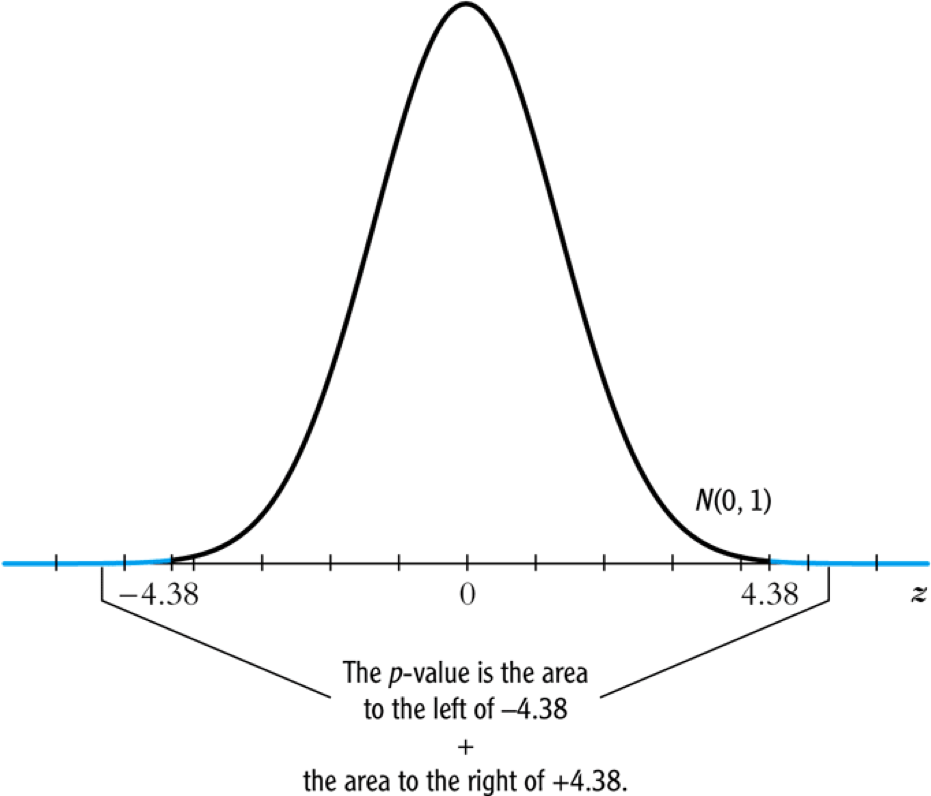
\includegraphics[width=0.7\textwidth]{figure/fig-5-1.png}
\caption{\label{fig:orgc5a34c7}
Calculating the p-value of a two-sided test when \(t^{act}=-4.38\)}
\end{figure}
\end{frame}

\subsection*{The one-sided alternative hypothesis}
\label{sec:orga1798dd}

\begin{frame}[label={sec:org6f22138}]{The one-sided hypotheses}
\begin{itemize}
\item In some cases, it is appropriate to use a one-sided hypothesis
test. For example, the superintendent of the California school
districts want to know whether an increase in class sizes has a
negative effect on test scores, that is, \(\beta_1 < 0\).

\item For such a test, we can set up the null hypothesis and the one-sided
alternative hypothesis as

\[ H_0: \beta_1 = \beta_{1,0} \text{ vs. } H_1: \beta_1 < \beta_{1,0} \]
\end{itemize}
\end{frame}

\begin{frame}[label={sec:org4c22398}]{The one-sided left-tail test}
\begin{itemize}
\item The t-statistic is the same as in a two-sided test
\[ t = \frac{\hat{\beta}_1 - \beta_{1,0}}{SE(\hat{\beta}_1)} \]

\item Since we test \(\beta_1 < \beta_{1,0}\), if this is true, the
t-statistics should be statistically significantly less than zero.

\item The p-value is computed as \(\mathrm{Pr}(t < t^{act}) = \Phi(t^{act})\).

\item The null hypothesis is rejected at the 5\% significance level when
\(\text{p-value} < 0.05\) or \(t^{act} < -1.645\).

\item In the application of test scores, the t-statistics is -4.38, which
is less than -1.645 and -2.33. Thus, the null hypothesis is rejected
at the 1\% level.
\end{itemize}
\end{frame}




\section*{Confidence Intervals for a Regression Coefficient}
\label{sec:org1ac622c}

\subsection*{Two equivalent definitions of confidence intervals}
\label{sec:org62167dd}

\begin{itemize}
\item Recall that a 95\% \alert{confidence interval} for \(\beta_1\) has two equivalent
definitions:
\begin{enumerate}
\item It is the set of values of \(\beta_1\) that cannot be rejected
using a two-sided hypothesis test with a 5\% significance level.
\item It is an interval that has a 95\% probability of containing the true
value of \(\beta_1\).
\end{enumerate}
\end{itemize}

\subsection*{Construct the 95\% confidence interval for \(\beta_1\)}
\label{sec:org39f1c31}

\begin{itemize}
\item We can obtain the 95\% confidence interval for \(\beta_1\) using the t
statistic and the acceptance region at the 5\% significant level.

\item The acceptance region is \(-1.96 \leq \frac{\hat{\beta}_1 - \beta_1}{SE(\hat{\beta}_1)} \leq 1.96\)

\item The 95\% confidence interval for \(\beta_1\) is
\[ \left[ \hat{\beta}_1 - 1.96 SE(\hat{\beta}_1),\; \hat{\beta}_1 + 1.96
  SE(\hat{\beta}_1) \right] \]
\end{itemize}

\subsection*{The application to test scores}
\label{sec:orgf8980c1}

\begin{itemize}
\item In the application to test scores, given that \(\hat{\beta}_1 = -2.28\)
and \(SE(\hat{\beta}_1) = 0.52\), the 95\% confidence interval for
\(\beta_1\) is
$${-2.28 \pm 1.96 \times 0.52}, \text{ or } -3.30 \leq \beta_1
  \leq -1.26$$

\item The confidence interval only spans over the negative region,
implying that the null hypothesis of \(\beta_1 = 0\) can be rejected
at the 5\% significance level.
\end{itemize}

\subsection*{Confidence intervals for predicted effects of changing \(X\)}
\label{sec:org33a0709}

\begin{itemize}
\item \(\beta_1\) is the marginal effect of \(X\) on \(Y\). That is, when \(X\)
changes by \(\Delta X\), \(Y\) changes by \(\beta_1 \Delta X\).

\item So the 95\% confidence interval for the change in \(Y\) when \(X\)
changes by \(\Delta X\) is
\begin{gather*}
\left[ \hat{\beta}_1 - 1.96 SE(\hat{\beta}_1)  ,\;
\hat{\beta}_1  + 1.96SE(\hat{\beta}_1) \right] \times \Delta X \\
= \left[ \hat{\beta}_1 \Delta X - 1.96 SE(\hat{\beta}_1) \Delta X,\;
\hat{\beta}_1 \Delta X + 1.96SE(\hat{\beta}_1) \Delta X \right]
\end{gather*}
\end{itemize}


\section*{Regression When \(X\) is a Binary Variable}
\label{sec:org8937ca8}

\subsection*{A binary variable}
\label{sec:org47a6f9e}

\begin{itemize}
\item A \alert{binary variable} takes on values of one if some condition is true
and zero otherwise, which is also called a \alert{dummy variable}, a
\alert{categorical variable}, or an \alert{indicator variable}.

\begin{equation*}
D_i =
\begin{cases}
1,\; &\text{if the } i^{th} \text{ subject is female} \\
0,\; &\text{if the } i^{th} \text{ subject is male}
\end{cases}
\end{equation*}
\end{itemize}

\subsection*{The linear regression model with a binary regressor}
\label{sec:org730ff51}

\begin{equation}
Y_i = \beta_0 + \beta_1 D_i + u_i,\; i = 1, \ldots, n
\end{equation}

\begin{itemize}
\item \(\beta_1\) is estimated by the OLS estimation method
in the same way as a continuous regressor.
\end{itemize}

\subsection*{Interpretation of the regression coefficients}
\label{sec:org19a9077}

\begin{itemize}
\item Given that the assumption \(E(u_i | D_i) = 0\) holds, we have two
population regression functions:
\begin{itemize}
\item When \(D_i = 1\), \(E(Y_i|D_i = 1) = \beta_0 + \beta_1\)
\item When \(D_i = 0\), \(E(Y_i|D_i = 0) = \beta_0\)
\end{itemize}

\item \(\beta_1 = E(Y_i | D_i = 1) - E(Y_i |D_i = 0)\), i.e.,
\alert{the difference in the population means} between two groups.
\end{itemize}

\subsection*{Hypothesis tests and confidence intervals}
\label{sec:org3530403}

\begin{itemize}
\item The null v.s. alternative hypothesis

\[ H_0:\, \beta_1 = 0 \text{ vs. } H_1:\, \beta_1 \neq 0 \]

\item The t-statistic

\[ t = \frac{\hat{\beta}_1}{SE(\hat{\beta}_1)} \]

\item The 95\% confidence interval

\[ \hat{\beta}_1 \pm 1.96 SE(\hat{\beta}_1) \]
\end{itemize}

\subsection*{Application to test scores}
\label{sec:orge8f68ca}

\begin{itemize}
\item We use a binary variable \(D\) to represent small and large
classes. 

\begin{equation*}
D_i =
\begin{cases}
1,\; &\text{if } STR_i < 20 \text{ (small classes)} \\
0,\; &\text{if } STR_i \geq 20 \text{ (large classes)}
\end{cases}
\end{equation*}

\item Using the OLS estimation, the estimated regression function is
\begin{equation*}
\widehat{TestScore} = \underset{\displaystyle (1.3)}{650.0} -
\underset{\displaystyle (1.8)}{7.4} D,\; R^2 = 0.037,\; SER = 18.7
\end{equation*}
\end{itemize}

\begin{frame}[label={sec:orgd225677}]{Application to test scores (cont'd)}
\begin{itemize}
\item The t-statistic for \(\beta_1\) is \(t = 7.4 / 1.8 = 4.04 > 1.96\) so that
\(\beta_1\) is significantly different from zero. 
\begin{itemize}
\item The test score in small classes are on average 7.4 higher than that in
large classes.
\end{itemize}

\item The confidence interval for the difference is \(7.4 \pm
  1.96 \times 1.8 = (3.9, 10.9)\).
\end{itemize}
\end{frame}



\section*{Heteroskedasticity and Homoskedasticity}
\label{sec:org4a265d0}

\subsection*{Homoskedasticity}
\label{sec:orged4d80b}

\begin{itemize}
\item The error term \(u_i\) is \alert{homoskedastic} if the conditional variance of
\(u_i\) given \(X_i\) is constant for all \(i = 1, \ldots, n\).

\item Mathematically, it says \(\mathrm{Var}(u_i | X_i) = \sigma^2,\, \text{ for }
  i = 1, \ldots, n\), i.e., the variance of \(u_i\) for all \emph{i} is a
constant and does not depend on \(X_i\).
\end{itemize}

\subsection*{Heteroskedasticity}
\label{sec:orgdd8439b}

\begin{itemize}
\item The error term \(u_i\) is \alert{heteroskedastic} if the conditional variance of
\(u_i\) given \(X_i\) changes on \(X_i\) for \(i = 1, \ldots, n\).

\item \(\mathrm{Var}(u_i | X_i) = \sigma^2_i,\, \text{ for } i = 1, \ldots, n\).

\item A multiplicative form of heteroskedasticity is
\(\mathrm{Var}(u_i|X_i) = \sigma^2 f(X_i)\) where \(f(X_i)\) is a
function of \(X_i\), for example, \(f(X_i) = X_i\) as a simplest case.
\end{itemize}

\subsection*{Homoskedasticity and heteroskedasticity compared}
\label{sec:org14085d2}

\begin{figure}[htbp]
\centering
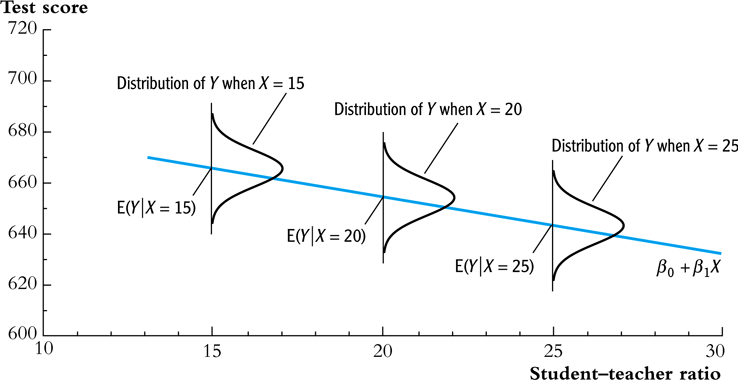
\includegraphics[width=.9\linewidth]{figure/fig-4-4.png}
\caption{Homoskedasticity}
\end{figure} 

\begin{figure}[htbp]
\centering
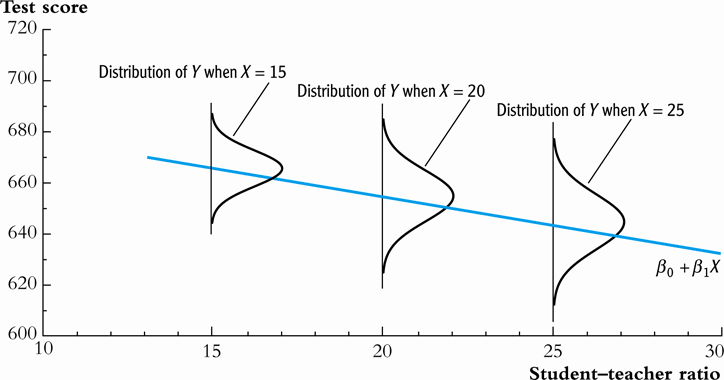
\includegraphics[width=.9\linewidth]{figure/fig-5-2.png}
\caption{Heteroskedasticity}
\end{figure}

Figure \ref{fig:homovshetero} for a visual comparison between
homoskedasticity and heteroskedasticity.

\begin{figure}
    \centering
    \begin{subfigure}[!ht]{0.85\textwidth}
        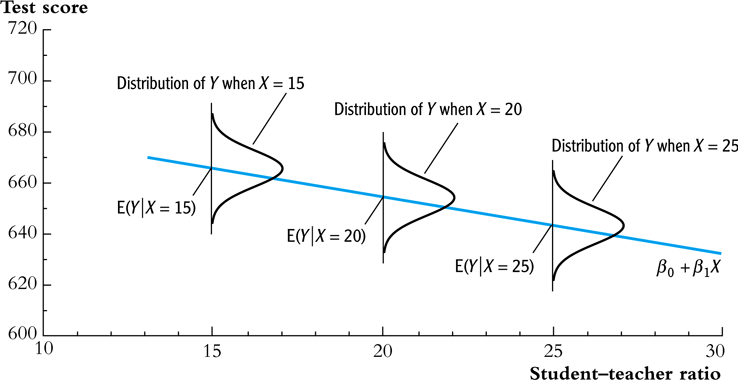
\includegraphics[width=\textwidth]{./figure/fig-4-4}
        \caption{Homoskedasticity}
        \label{fig:homo1}
    \end{subfigure}
    ~ %add desired spacing between images, e. g. ~, \quad, \qquad, \hfill etc.
      %(or a blank line to force the subfigure onto a new line)
    \begin{subfigure}[!ht]{0.85\textwidth}
        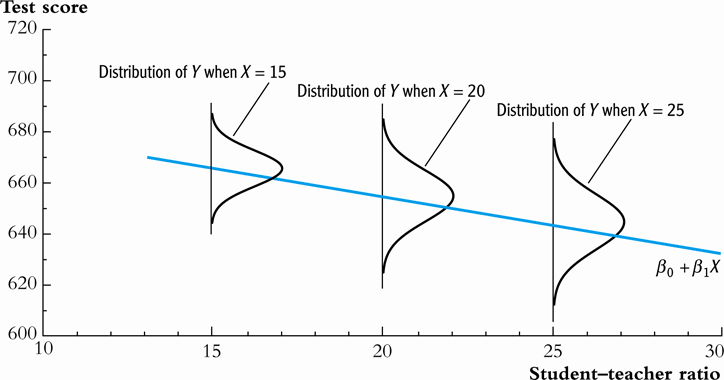
\includegraphics[width=\textwidth]{./figure/fig-5-2}
        \caption{Heteroskedasticity}
        \label{fig:hetero1}
    \end{subfigure}
    \caption{Homoskedasticity Versus Heteroskedasticity}\label{fig:homovshetero}
\end{figure}

\subsection*{Mathematical implications of homoskedasticity}
\label{sec:orgdaaaefe}

\begin{frame}[label={sec:org58612a6}]{Unbiasedness, consistency, and the asymptotic distribution}
\begin{itemize}
\item As long as the least squares assumptions holds, whether the error
term, \(u_i\), is homoskedastic or heteroskedastic does not affect
unbiasedness, consistency, and the asymptotic normal distribution
of the OLS estimators.
\begin{itemize}
\item The unbiasedness requires that \(E(u_i|X_i) = 0\)
\item The consistency requires that \(E(X_i u_i) = 0\), which is true if
\(E(u_i|X_i)=0\).
\item The asymptotic normal distribution requires additionally that
\(\mathrm{Var}((X_i-\mu_X)u_i) < \infty\), which still holds as long as
Assumption 3 holds.
\end{itemize}
\end{itemize}
\end{frame}

\begin{frame}[label={sec:orgc20e26e}]{Efficiency}
\begin{itemize}
\item The existence of heteroskedasticity affects the enfficiency of the
OLS estimator

\begin{itemize}
\item Suppose \(\hat{\beta}_1\) and \(\tilde{\beta}_1\) are both unbiased
estimators of \(\beta_1\). Then, \(\hat{\beta}_1\) is said to be more
\alert{efficient} than \(\tilde{\beta}_1\) if 
$$\mathrm{Var}(\hat{\beta}_1) < \mathrm{Var}(\tilde{\beta}_1)$$

\item When the errors are homoskedastic, the OLS estimators
\(\hat{\beta}_0\) and \(\hat{\beta}_1\) are the most efficient among
all estimators that are linear in \(Y_1, \ldots, Y_n\) and are
unbiased, conditional on \(X_1, \ldots, X_n\).
\end{itemize}
\end{itemize}
\end{frame}

\subsection*{The homoskedasticity-only variance formula}
\label{sec:org01f5553}

\begin{itemize}
\item Recall that we can write \(\hat{\beta}_1\) as
\begin{equation*}
\hat{\beta}_1 = \beta_1 + \frac{\sum_i (X_i - \bar{X})u_i}{\sum_i
(X_i - \bar{X})^2}
\end{equation*}

\item If \(u_i\) for \(i=1, \ldots, n\) is homoskedastic and \(\sigma^2\) is
known, then
\begin{equation}
\label{eq:vbeta-1a} 
\sigma^2_{\hat{\beta}_1} = \mathrm{Var}(\hat{\beta}_1 | X_i) = \frac{\sum_i (X_i -
\bar{X})^2 \mathrm{Var}(u_i|X_i)}{\left[\sum_i (X_i - \bar{X})^2\right]^2} =
\frac{\sigma^2}{\sum_i (X_i - \bar{X})^2}
\end{equation}
\end{itemize}

\begin{frame}[label={sec:org97cf9ab}]{The homoskedasticity-only variance when \(\sigma^2\) is unknown}
\begin{itemize}
\item When \(\sigma^2\) is unknown, then we use \(s^2_u = 1/(n-2) \sum_i
  \hat{u}_i^2\) as an estimator of \(\sigma^2\).

\item The homoskedasticity-only estimator of the variance of \(\hat{\beta}_1\) is
\begin{equation}
\label{eq:vbeta-1b} \tilde{\sigma}^2_{\hat{\beta}_1} =
\frac{s^2_u}{\sum_i (X_i - \bar{X})^2}
\end{equation}

\item The homoskedasticity-only standard error is \(SE(\hat{\beta}_1) =
  \sqrt{\tilde{\sigma}^2_{\hat{\beta}_1}}\).
\end{itemize}
\end{frame}

\begin{frame}[label={sec:org4abe2e8}]{The heteroskedasticity-robust standard error}
\begin{itemize}
\item The heteroskedasticity-robust standard error is
\begin{equation*}
SE(\hat{\beta}_1) = \sqrt{\hat{\sigma}^2_{\hat{\beta}_1}}
\end{equation*}
where
\begin{equation*}
\hat{\sigma}^2_{\hat{\beta}_1} = \frac{1}{n} \frac{\frac{1}{n-2}
\sum_{i=1}^n (X_i - \bar{X})^2 \hat{u}^2_i}{\left[ \frac{1}{n}
\sum_{i=1}^n (X_i - \bar{X})^2 \right]^2}
\end{equation*}
which is also referred to as Eicker-Huber-White standard errors.
\end{itemize}
\end{frame}

\subsection*{What does this mean in practice?}
\label{sec:orgffd09b2}

\begin{itemize}
\item Heteroskedasticity is common in cross-sectional data. It is always
safer to report the heteroskedasticity-robust standard errors and
use these to compute the robust t-statistic.

\item In most software, the default setting is to report the
homoskedasticity-only standard errors. Therefore, you need to
manually add the option for the robust estimation.

\begin{itemize}
\item In R, you can use the following codes
\begin{verbatim}
library(lmtest)
model1 <- lm(testscr ~ str, data = classdata)
coeftest(model1, vcov = vcovHC(model1, type="HC1"))
\end{verbatim}
\end{itemize}
\end{itemize}




\section*{The Theoretical Foundations of Ordinary Least Squares}
\label{sec:orgfa112f2}

\subsection*{The Gauss-Markov conditions}
\label{sec:org2d9de27}

\begin{frame}[label={sec:org11d293d}]{The least squares assumptions}
\begin{itemize}
\item We have already known the least squares assumptions: 

for \(i = 1, \ldots, n\), 

\begin{enumerate}
\item \(E(u_i|X_i) = 0\)
\item \((X_i, Y_i)\) are i.i.d., and
\item Large outliers are unlikely.
\end{enumerate}
\end{itemize}
\end{frame}

\begin{frame}[label={sec:org5ae1fc2}]{The Gauss-Markov conditions}
For \(\mathbf{X} = [X_1, \ldots, X_n]\)

\begin{enumerate}
\item \(E(u_i| \mathbf{X}) = 0\) (The exogeneity assumption )
\item \(\mathrm{Var}(u_i | \mathbf{X}) = \sigma^2_u,\, 0 < \sigma^2_u < \infty\)
(The homoskedasticity assumption)
\item \(E(u_i u_j | \mathbf{X}) = 0,\, i \neq j\) (The uncorrelation assumption)
\end{enumerate}
\end{frame}

\begin{frame}[label={sec:org8390062}]{From the three Least Squares Assumptions and the homoskedasticity assumption to the Gauss-Markov conditions}
\begin{itemize}
\item All the Gauss-Markov conditions, except for  the homoskedasticity
assumption, can be derived from the least squares assumptions.
\begin{itemize}
\item The least squares assumptions (1) and (2) imply \(E(u_i | \mathbf{X}) =
    E(u_i | X_i) = 0\).
\item The least squares assumptions (1) and (2) imply \(\mathrm{Var}(u_i|
    \mathbf{X}) = \mathrm{Var}(u_i | X_i)\).
\item With the homoskedasticity assumption, \(\mathrm{Var}(u_i | X_i) =
    \sigma^2_u\), the least squares assumption (3) then implies \(0 < \sigma^2_u <
    \infty\).
\item The least squares assumptions (1) and (2) imply that \(E(u_i u_j |
    \mathbf{X}) = E(u_i u_j | X_i, X_j) = E(u_i|X_i) E(u_j|X_j) = 0\).
\end{itemize}
\end{itemize}
\end{frame}

\subsection*{The Gauss-Markov Theorem}
\label{sec:orgf1febcb}

\begin{itemize}
\item The Gauss-Markov Theorem for \(\hat{\beta}_1\):

If the Gauss-Markov conditions hold, then the OLS estimator
\(\hat{\beta}_1\) is the Best (most efficient) Linear conditionally
Unbiased Estimator (BLUE).

\item The theorem can also be applied to \(\hat{\beta}_0\).
\end{itemize}

\subsection*{Linear conditionally unbiased estimator}
\label{sec:org7e227f9}

\begin{frame}[label={sec:orge81cb9b}]{The linear estimators of \(\beta_1\)}
\begin{itemize}
\item Any linear estimator \(\tilde{\beta}_1\), it can be written as
\begin{equation}
\label{eq:beta1-tilde}
\tilde{\beta}_1 = \sum_{i=1}^n a_i Y_i\
\end{equation}
where the weights \(a_i\) for \(i = 1, \ldots, n\) depend on \(X_1, \ldots,
  X_n\) but not on \(Y_1, \ldots, Y_n\).
\end{itemize}
\end{frame}

\begin{frame}[label={sec:orgf73f69c}]{The linear conditionally unbiased estimators}
\begin{itemize}
\item \(\tilde{\beta}_1\) is conditionally unbiased means that
\begin{equation}
\label{eq:e-beta1-tilde}
E(\tilde{\beta}_1 | \mathbf{X}) = \beta_1\
\end{equation}

\item By the Gauss-Markov conditions, we can have
\begin{equation*}
\begin{split}
E(\tilde{\beta}_1 | \mathbf{X}) &= \sum_i a_i E(\beta_0 + \beta_1 X_i + u_i | \mathbf{X}) \\
&= \beta_0 \sum_i a_i + \beta_1 \sum_i a_i X_i
\end{split}
\end{equation*}

\item For the equation above being satisfied with any
\(\beta_0\) and \(\beta_1\), we must have
\[ \sum_i a_i = 0 \text{ and } \sum_i a_iX_i = 1 \]
\end{itemize}
\end{frame}

\begin{frame}[label={sec:orgc70bbc0}]{The OLS esimator \(\hat{\beta}_1\) is a linear conditionally unbiased estimator}
\begin{itemize}
\item \(\hat{\beta}_1 = \frac{\sum_i (X_i - \bar{X})(Y_i - \bar{Y})}{\sum_i
  (X_i - \bar{X})^2} = \frac{\sum_i (X_i - \bar{X})Y_i}{\sum_i (X_i -
  \bar{X})^2} = \sum_i \hat{a}_i Y_i\)

where the weights are
\[ \hat{a}_i = \frac{X_i - \bar{X}}{\sum_i (X_i - \bar{X})^2}, \text{
  for } i = 1, \ldots, n \]

\item Since \(\hat{\beta}_1\) is a linear conditionally unbiased estimator, we
must have

\[ \sum_i \hat{a}_i = 0 \text{ and } \sum_i \hat{a}_i X_i = 1  \]

which can be simply verified.
\end{itemize}
\end{frame}

\subsection*{A scratch of the proof of the Gauss-Markov theorem}
\label{sec:org0324fe3}

\begin{itemize}
\item A key in the proof of the Gauss-Markov theorem is that we can
rewrite the expression of any linear conditionally unbiased
estimator \(\tilde{\beta}_1\) as
\[ \tilde{\beta}_1 = \sum_i a_i Y_i = \sum_i (\hat{a}_i + d_i)Y_i =
  \hat{\beta}_1 + \sum_i d_i Y_i \]
\item The goal of
the proof is to show that
\[ \mathrm{Var}(\hat{\beta}_1 | \mathbf{X}) \leq \mathrm{Var}(\tilde{\beta}_1 |
  \mathbf{X}) \]
The equality holds only when \(\tilde{\beta}_1 = \hat{\beta}_1\).

\item The proof of the Gauss-Markov theorem is in Appendix 5.2.
\end{itemize}

\subsection*{The limitations of the Gauss-Markov theorem}
\label{sec:org938d375}

\begin{itemize}
\item The Gauss-Markov conditions may not hold in practice.

\item Any violation of the Gauss-Markov conditions will result in the OLS
estimators that are not BLUE.

\begin{table}[htbp]
\caption{Summary of Violations of the Gauss-Markov Theorem}
\centering
\small
\begin{tabular}{p{4cm}|p{5.5cm}|p{2.5cm}|p{3.4cm}}
\toprule
Violation & Cases & Consequences & Remedies\\
\midrule
\(E(u \mid X) \neq 0\) & omitted variables, endogeneity & biased & more \(X\), IV method\\
\(\mathrm{Var}(u_i\mid X)\) not constant & heteroskedasticity & inefficient & WLS, GLS, HCCME\\
\(E(u_{i}u_{j}\mid X) \neq 0\) & autocorrelation & inefficient & GLS, HAC\\
\bottomrule
\end{tabular}
\end{table}
\end{itemize}



\section*{Using the t-Statistic in Regression When the Sample Size is Small}
\label{sec:orga798250}

\subsection*{The classical assumptions of the least squares estimation}
\label{sec:org58ce979}

\begin{itemize}
\item The classical assumptions of the least squares estimation:

For \(i = 1, 2, \ldots, n\)
\begin{itemize}
\item Assumption 1: \(E(u_i | X_i) = 0\) (exogeneity of \(X\))
\item Assumption 2: \((X_i, Y_i)\) are i.i.d. (IID of \(X, Y\))
\item Assumption 3: \(0 < E(X_i^4) < \infty\) and \(0 < E(Y_i^4) < \infty\)
(No large outliers)
\item Extended Assumption 4: \(\var(u_i | X_i) = \sigma^2_u, \text{ and } 0 <
                     \sigma^2_u < \infty\) (homoskedasticity)
\item Extended Assumption 5: \(u_i | X_i \sim N(0, \sigma^2_u)\) (normality)
\end{itemize}
\end{itemize}


\subsection*{The t-Statistic and the Student-t Distribution}
\label{sec:org4b8dc61}

\begin{frame}[label={sec:orgcc17df0}]{The t-statistic is for \(\beta_1\)}
\[H_0: \beta_1 = \beta_{1,0} \text{ vs } H_1: \beta_1 \neq \beta_{1,0}\]
\begin{equation}
t = \frac{\hat{\beta}_1 - \beta_{1,0}}{\hat{\sigma}_{\hat{\beta}_1}}
\end{equation}
where
\begin{equation*}
\hat{\sigma}^2_{\hat{\beta}_1} = \frac{s^2_u}{\sum_i (X_i - \bar{X})^2} \text{ and } s^2_u = \frac{1}{n-2}\sum_i \hat{u}_i^2 = SER^2
\end{equation*}
the former of which is the homoskedasticity-only standard error of
\(\hat{\beta}_1\) and the latter is the standard error of the
regression.
\end{frame}



\begin{frame}[label={sec:org6b6c4c1}]{The Student-t distribution of \(t\)}
\begin{itemize}
\item When the classical least squares assumptions hold, the
t-statistic has the exact distribution of \(t(n-2)\), i.e., the
Student's t distribution with \((n-2)\) degrees of freedom.

\[ t = \frac{\hat{\beta}_1 -
  \beta_{1,0}}{\hat{\sigma}_{\hat{\beta}_1}} \sim t(n-2) \]
\end{itemize}
\end{frame}
\end{document}